\documentclass[11 pt]{report}
\usepackage{structure}

\title{{\Huge Numerical simulation of yield stress fluid flows with X-MESH}}
\author{\textsc{DEGROOFF} Vincent}
\date{\today}


\begin{document}
 
%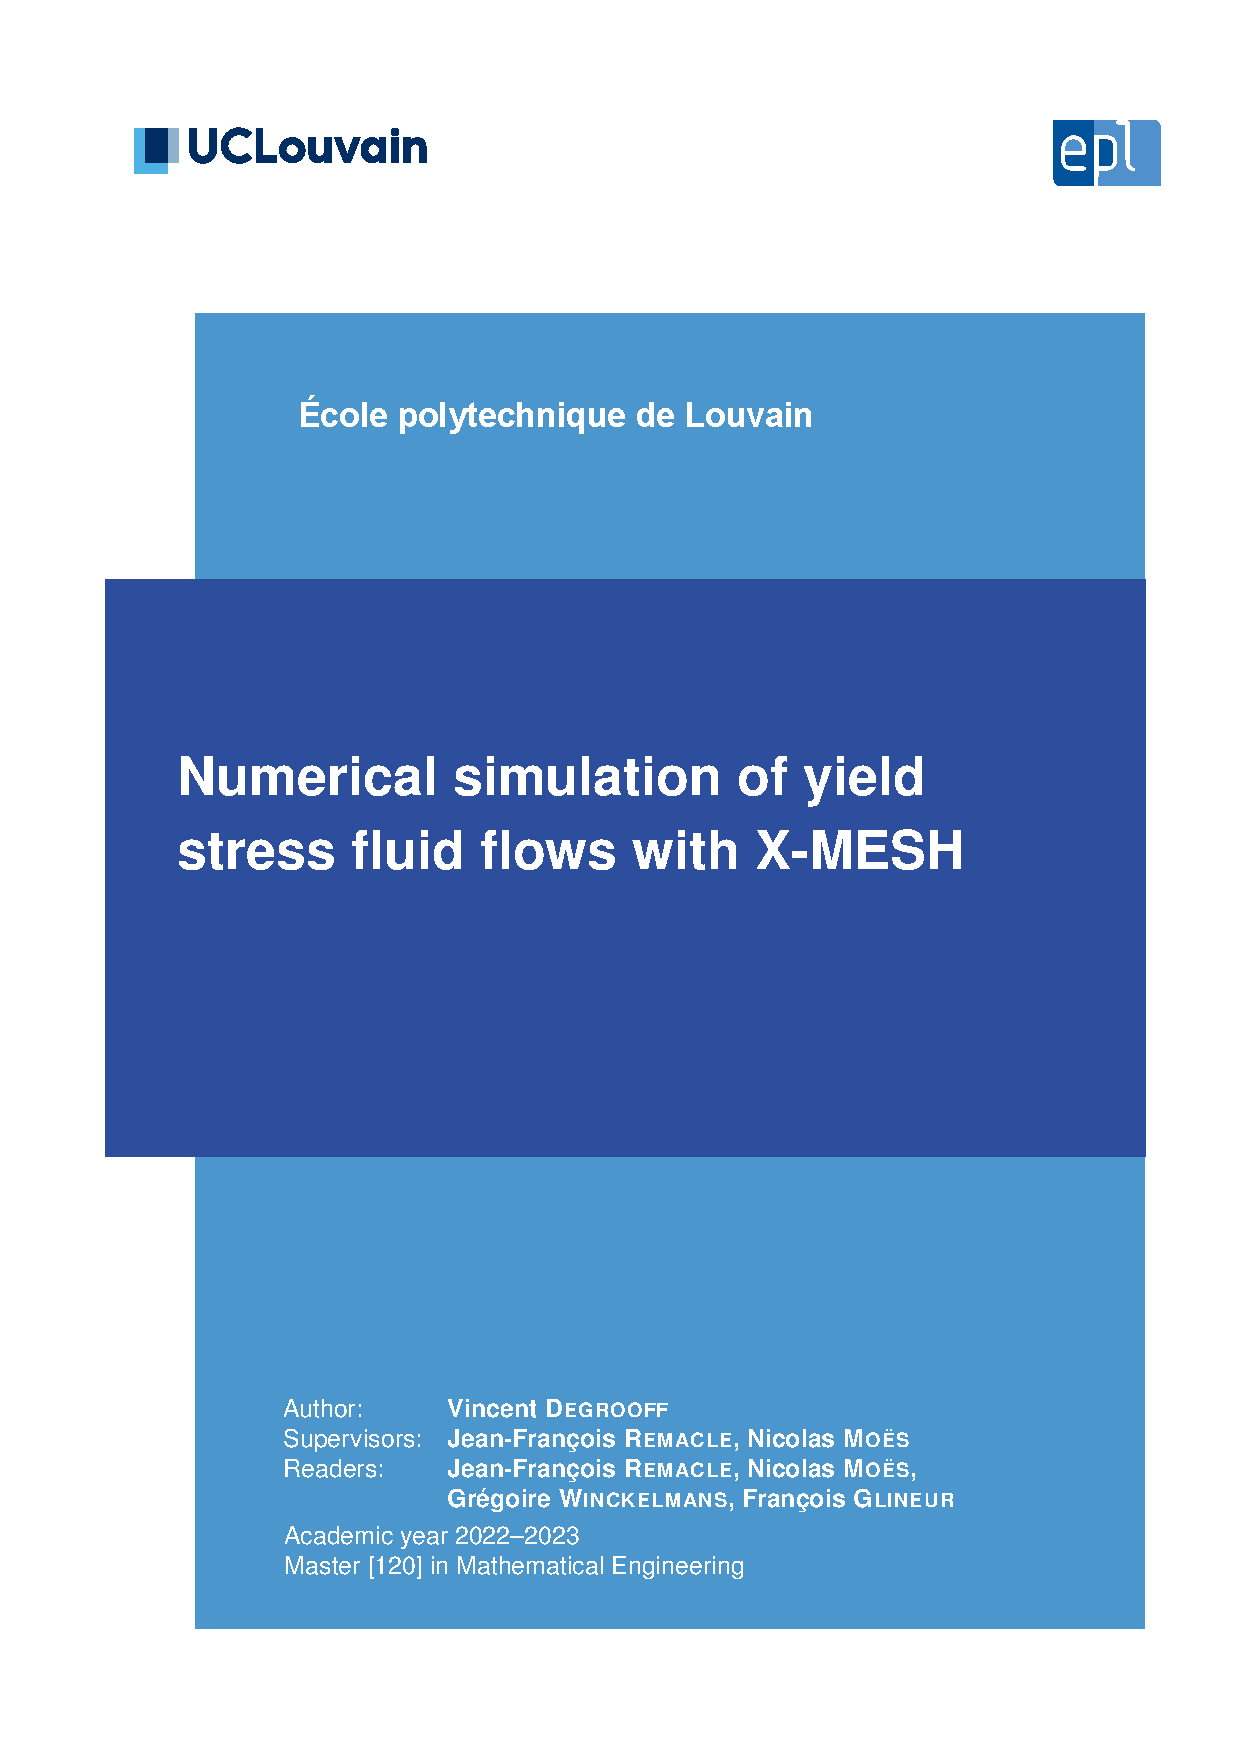
\includepdf[pages=-]{front_page.pdf}
\maketitle

\setcounter{tocdepth}{1}
\tableofcontents

% FOR introduction
%The flow characteristics of such materials are difficult to predict as they involve [...] solid and liquid regions that are generally impossible to locate a priori. CITE Coussot if used so  -->  use X-MESH

% Index i: element
% Index j: node
% Index e: edge
% Index g: gauss point

\addcontentsline{toc}{chapter}{Introduction}
\chapter*{Introduction}
An introduction

\chapter{Governing equations}

\section{General notions of continuum mechanics}
Let $\Omega \in \mathbb{R}^3$ denote the domain of interest and $\Gamma=\partial \Omega$ its boundary. Let $\mathbf{u}$ be the fluid velocity, and $\boldsymbol{\sigma}=-p\mathbf{I}+\boldsymbol{\tau}$ be the stress tensor with its deviatoric contribution $\boldsymbol\tau$.

Let us recall the mass and momentum conservation equations, with the pressure $p$ and body forces $\mathbf{f}$, expressed in an Eulerian reference frame:
\begin{align}
    \nabla \cdot \mathbf{u} &= 0\\
    \rho \left(\pdv{\mathbf{u}}{t} + \left(\mathbf{u} \cdot \nabla\right) \mathbf{u}\right) &= -\nabla p + \nabla \cdot \boldsymbol\tau + \mathbf{f}
\end{align}

%In both yielded and unyielded regions, the stress tensor is continuous (\textcolor{red}{seems obvious, in the yielded zones, but what about the solid part ?}). At the interface, the conservation of mass and momentum read as follows, where $[\![ . ]\!]$ refers to the difference of the fields across the interface and $\mathbf{u^*}$ to the interface velocity:
% \begin{align}
%     [\![ \rho (\mathbf{u^* - \mathbf{u}}) \cdot \mathbf{\hat n} ]\!] &= 0 \label{eq:interface_mass}\\
%     [\![ \rho \mathbf{u} (\mathbf{u^* - \mathbf{u}}) \cdot \mathbf{\hat n} + \mathbf{\hat n} \cdot \sigma ]\!] &= 0 \label{eq:interface_momentum}
% \end{align}

Throughout this study, we will consider low Reynolds numbers, i.e. flows that are dominated by viscous forces. We will thus neglect the inertia terms on the left of equation \eqref{eq:momentum}. The resulting equations are the well known Stokes equations, where we look for velocity and pressure fields $(\uu,p)$ solution of
\begin{empheqboxed}
    \begin{align}
        0 &= -\nabla p + \nabla \cdot \boldsymbol \tau(\uu) + \mathbf{f} &&\text{in} \; \Omega \label{eq:momentum} \\[2pt]
        0 &= \nabla \cdot \uu &&\text{in}\; \Omega \label{eq:mass}\\[6pt]
        \uu &= \mathbf{U} &&\text{on}\; \Gamma_{D} \label{eq:Dirichlet}\\[2pt]
        \boldsymbol \sigma \cdot \nn &= \mathbf{g} &&\text{on}\; \Gamma_{N} \label{eq:Neumann}
    \end{align}
\end{empheqboxed}
where $\Gamma_{D}$ and $\Gamma_{N}$ refer to the partitions of $\partial \Omega$ where Dirichlet and Neumann boundary conditions are applied. $\mathbf{U}$ and $\mathbf{g}$ are given beforehand. One could also decide to impose only the normal velocity along with the tangential stress, or the tangential velocity along with the normal stress, as will be explained in more detail in \cref{sec:boundary_conditions}.

Before looking for a closure equation for the shear stress tensor, let us first recall the velocity gradient decomposition,
\begin{empheqboxed}
    \begin{align}
        \nabla \mathbf{u} &= \mathbf{D} + \mathbf{W}\\[4pt]
        \mathbf{D} &= \frac{1}{2} \left(\nabla \mathbf{u} + \nabla^T \mathbf{u}\right) = \frac{1}{2} \gam\\[4pt]
        \mathbf{W} &= \frac{1}{2} \left(\nabla \mathbf{u} - \nabla^T \mathbf{u}\right)
    \end{align}
\end{empheqboxed}

To be exhaustive:
\begin{itemize}[label=---]
    \item $\mathbf{D}$ is the strain-rate tensor, whose diagonal elements indicate the stretching of the fluid along the basis vectors and whose off-diagonal elements indicate the shearing of the fluid from one basis vector to another.
    \item $\mathbf{W}$ is the spin tensor that indicates the axis around which the flow is locally rotating, as well as the speed of this rotation.
\end{itemize} 

\section{Constitutive equations of Bingham fluids}

Newtonian fluid behavior is the most simple one can find in fluid mechanics because it assumes that the fluid deformation, or strain rate, is is directly proportional to the shear stress it undergoes. It is very accurate for many liquids and gases such as air, water, gasoline or alcohol, under normal conditions. However, this model cannot characterize a variety of well known substances from blood to toothpaste to ketchup to name a few.

Such fluids are much better described as \textit{generalized Newtonian} \cite{Geophysical}. This model extends Newtonian fluids with a nonlinear constitutive law between the stress $\boldsymbol\tau$ and strain rate $\gam$:
\begin{equation}
    \boldsymbol\tau = \mu(\gam, T, \phi) \gam
    \label{eq:power-law}
\end{equation}
where $\mu$, $T$ and $\phi$ respectively refer to the fluid viscosity, the temperature and the particle concentration (e.g. polymer chains in dilute solutions). Since the viscosity, a scalar, depends on the tensor $\gam$, then it must depend only on the combinations of components $\gamma_{ij}$ that are not dependent on the coordinate system \cite{bird1987dynamics}. These combinations are the tensor invariants, described below and intimately connected to its eigenvalues $\lambda_i$, as one can find by diagonalizing the matrix $\gam$.
\begin{equation}
    \begin{alignedat}{2}
        I_1(\gam) &\coloneqq \Tr(\gam) &&= \lambda_1 + \lambda_2 + \lambda_3\\
        I_2(\gam) &\coloneqq \frac{1}{2} \left[\big(\Tr(\gam)\big)^2 - \Tr(\gam \cdot \gam)\right] &&= \lambda_1\lambda_2 + \lambda_2\lambda_3 + \lambda_3\lambda_1\\
        I_3(\gam) &\coloneqq \det(\gam) &&= \lambda_1\lambda_2\lambda_3
    \end{alignedat}
\end{equation}

The first invariant is always zero when we deal with incompressible fluids since $\Tr(\gam) = 2 \nabla \cdot \vv$. The third invariant is always neglected because it is also zero for shearing flows in 3 dimensions -- $\vv = u(y)\mathbf{e}_1$ -- precisely those for which the theory was developed. The constitutive law was then later used to model more complex flows, but the absence of $I_3$ has persisted \cite{bird1987dynamics}.

The simplest example of Generalized Newtonian fluids are the Power-law Fluids, that assume $\mu(\dot\gamma) = K \dot \gamma^{n-1}$, with the \textit{consistency} $K$ and \textit{index} $n$. This can already describe
\begin{itemize}[label=---, topsep=0pt]
    \setlength{\itemsep}{0pt}
    \item\textit{Shear thinning} fluids with viscosity inversely proportional to strain rate $(n<1)$. For example, Ketchup or blood flow more easily with higher strain rates.
    \item\textit{Shear thickening} or \textit{Dilatant} fluids with viscosity proportional to strain rate $(n>1)$. A typical example is the mixture of cornstarch and water, called Oobleck, that appears liquid at rest, but that becomes viscous enough to walk on it if struck hard enough.
    \item \textit{Newtonian} fluids of course when $n=1$.
\end{itemize}

However, this model is not sufficient to describe certain fluids under low shear stress. For example, the toothpaste flows like a liquid out of the tube, but stays in its configuration once on the toothbrush, so we can easily put it in our mouth without dropping any on the floor: at low stress, such a fluid is considered to behave as a solid.

The Herschel-Bulkley Model extends the Power-law model with a yield stress $\tau_0$, that enables us to simulate yield stress fluids like the toothpaste. When the shear stress tensor norm $\tau < \tau_0$, the fluid behaves as a non-deformable solid ($\gam=\mathbf{0}$) and is called \textit{unyielded}. In these regions, the fluid undergoes a rigid-body motion: a uniform translation and/or a uniform rotation, or possibly at rest.

Above that threshold, the fluid becomes \textit{yielded} and follows the Power-law model. The constitutive law of the Herschel-Bulkley Model reads as follows
\begin{equation}
    \begin{aligned}
        \dot \gamma_{ij} &= 0 & \text{if} \quad \tau \leq \tau_0\\
        \tau_{ij} &= \left(K \dot \gamma^{n-1} + \frac{\tau_0}{\dot \gamma}\right) \gamma_{ij} & \text{if} \quad \tau \geq \tau_0\\
    \end{aligned}
    \label{eq:herschel}
\end{equation}
where $\dot \gamma$ and $\tau$ are the square root the second invariant tensor of $\gam$ and $\boldsymbol\tau$, also equal to their Frobenius norm since they are traceless:
\begin{equation}
    \dot \gamma \coloneqq \sqrt{|I_2(\gam)|} = \sqrt{\frac{1}{2} \, \gam : \gam} = \sqrt{2 \mathbf{D} : \mathbf{D}} \qquad\text{and}\qquad
    \tau \coloneqq \sqrt{|I_2(\boldsymbol\tau)|} = \sqrt{\frac{1}{2} \, \boldsymbol\tau : \boldsymbol\tau}
    \label{eq:tensornorm}
\end{equation}


\begin{figure}[t]
    \centering
    \includesvg[width=\textwidth]{../figures/fluid_classification.svg}
    \caption{Non-Newtonian fluid models.}
    \label{fig:fluid-classification}
\end{figure}

Common values of $n$ generally lies between $0.3$ and $0.5$, especially for Carbopol gels (e.g. hair gel) and emulsions (e.g. mustard, mayonnaise). The Bingham model ($n = 1$) is thus very rarely obtained when it is fitted over more than two orders of magnitude of shear rates. The yield stress value $\tau_0$ generally lies in the range [1, 100 Pa]. \cite{Coussot}. To give a feel of how common substances fit in this model, several sets of parameters are provided in \cref{tab:parameters}.

Those values are not universal. It is in fact hard to find unanimous parameters values of the Herschel-Bulkley model in the literature, especially for food products because their composition may depend on the brand, e.g. the yield stress of mayonnaise is inversely proportional to its fat content \cite{mayonnaiseFat}. The values may also depend on the test methodology, and on the model for which the experimental data is fitted, which is not always Herschel-Bulkley.

\begin{table}[t]
    \centering
    \begin{tabular}[t]{lccc}
        \toprule
        Substance 
        & Yield stress $\tau_0$ $[\mathrm{Pa}]$ 
        & Consistency $K$ $[\mathrm{Pa \, s^n}]$ 
        & Index $n$ $[-]$\\
        \midrule
        Ketchup \cite{ketchup}       & 13 -- 32 & 2--6 & 0.44 -- 0.62 \\[2pt]
        Mayonnaise \cite{mayonnaise1,mayonnaise2} & 75 -- 200 & 10 -- 50 & 0.4 -- 0.65 \\[2pt]
        Molten chocolate at $40^\circ C$ \cite{chocolate} & 8 & 2.4 & 0.88 \\[2pt]
        Hair gel \cite{gel}                     & 60 & 25 & 0.4 \\[2pt]
        \multirow{2}{*}{Toothpaste\cite{toothpaste}}
                                     & $\sim 50$ for children & . & . \\
                                     & $\sim 220$ for adults & . & . \\[2pt]
        Blood \cite{Lee2011}         & $32.5\times 10^{-3}$ & 5.62 & 0.955 \\[2pt]
        \bottomrule
    \end{tabular}
    \caption{Herschel-Bulkley parameters for common substances.}
    \label{tab:parameters}
\end{table}%

The present study will focus on simple yield stress fluids. By simple yield stress fluids are meant those for which the \textbf{shear stress depends only} on the imposed \textbf{shear rate}, and not on time (thixotropic/rheopectic) or shear (elastic behavior) \cite{simpleyield}. Thixotropic fluids have the property that their viscosity \textit{under constant shear} decreases with time. Though less common, rheopectic are the exact opposite where viscosity increases with time. This history dependence is also called \textit{hysteresis}, and such fluids can thus have an hysteresis loop in their stress-strain diagram. 

% INTRODUCTION
Furthermore, only Bingham fluids ($n=1$), will be considered hereafter. The equations of this model are indeed simpler to solve, but still provide solutions with the desired features that make them interesting to analyze with the X-MESH method. Let us then reformulate model \eqref{eq:herschel} for $n=1$, with $\dot\gamma$ defined in \eqref{eq:tensornorm}:
\begin{empheqboxed}
    \begin{equation}
        \begin{aligned}
            \|\boldsymbol\tau\| &< \tau_0 & \text{if} \quad \gam = \mathbf{0} \\ %\label{eq:tensor_unyielded}
            \boldsymbol{\tau} &= \left(K + \frac{\tau_0}{\dot \gamma}\right) \gam & \text{if} \quad  \gam \neq \mathbf{0} %\label{eq:tensor_yielded}
        \end{aligned}
        \label{eq:constitutive}
    \end{equation}
\end{empheqboxed}

\section{Weak formulation}
In order to solve \cref{eq:momentum,eq:mass} with the finite element method one can express them under its weak form. This is done by multiplying the equations of the strong form by velocity and pressure test functions $\vv$ and $q$. The shear stress tensor $\boldsymbol\tau$ is eventually replaced with its constitutive law \cref{eq:constitutive}.

\begin{equation}
    \begin{aligned}
        0 &= {\color{blue}-\nabla p} + {\color{red} \nabla \cdot \taub(\uu)} + \ff\\
        &= {\color{blue} \int_{\Omega} - \vv \cdot \nabla p \;\dd x} + {\color{red} \int_{\Omega} \vv \cdot (\nabla \cdot \taub) \;\dd x} + \int_{\Omega} \ff \cdot \vv  \;\dd x\\
        &= {\color{blue} \int_{\Omega} p \nabla \cdot \vv - \int_{\Omega} \nabla \cdot (p\vv)} + {\color{red} \int_{\Omega} \nabla \cdot (\taub \cdot \vv) - \int_{\Omega}  \taub (\uu) : \nabla^\top \vv} + \int_{\Omega} \ff \cdot \vv\\
        &= {\color{blue} \int_{\Omega} p \nabla \cdot \vv - \int_{\partial \Omega} p \vv \cdot \nn} + {\color{red} \int_{\partial\Omega} (\taub \cdot \vv) \cdot \nn - \int_{\Omega}  \taub (\uu) : \big(\mathbf{D}(\vv) + \mathbf{\Omega}(\vv)\big)^\top} + \int_{\Omega} \ff \cdot \vv \\
        &= {\color{blue} \int_{\Omega} p \nabla \cdot \vv \;\dd x} - {\color{red} \int_{\Omega}  \taub (\uu) : \mathbf{D}(\vv) \;\dd x} + \int_{\Omega} \ff \cdot \vv \;\dd x + {\color{violet}\int_{\Gamma_N} \mathbf{g} \cdot \vv \; \dd s}\\
        &= {\color{blue} \int_{\Omega} p \nabla \cdot \vv \;\dd x} - {\color{red} \int_{\Omega}  \left( 2K + \frac{\tau_0}{\|\mathbf{D}(\uu)\|} \right) \mathbf{D}(\uu) : \mathbf{D}(\vv) \;\dd x} + \int_{\Omega} \ff \cdot \vv \;\dd x + {\color{violet}\int_{\Gamma_N} \mathbf{g} \cdot \vv \; \dd s}
    \end{aligned}\label{eq:weak_formulation}
\end{equation}
that must hold $\forall \; \vv \in H^1(\Omega)^d$ such that $\vv = \mathbf{0} \text{ on } \Gamma_D$.

In \cref{eq:weak_formulation}, we initially multiplied \autoref{eq:momentum} by a test function $\mathbf{v}$ that is zero on $\Gamma_D$, then and integrated it over $\Omega$. Afterwards, we integrated by parts, used the Divergence theorem, and the property that the double contraction of symmetric and antisymmetric tensors cancels out.

On the other hand, \autoref{eq:mass} gets multiplied by a pressure test function $q$.
\begin{equation}
    \begin{aligned}
        \int_{\Omega} q \nabla \cdot \uu &= 0  && \forall q \in L^2(\Omega)
    \end{aligned}
    \label{eq:weak_formulation_p}
\end{equation}


\section{Energy functional}

The velocity field $\uu$ solution of this weak formulation can also be found through an energy functional $\mathcal{J}(\vv)$ \cite{Saramito, Bleyer}. As viscous forces dominate the physics of the problem, we can assume that viscous dissipation is the only source of internal energy. As in linear elasticity for solids, the infinitesimal work of internal stresses in the deformation is
\begin{equation}
    \begin{aligned}
        W_{\textrm{internal}}(D_{ij}) &= \int_{0}^{D_{ij}} \sigma_{ij} \:\dd D_{ij}'\\
        &= \int -p\delta_{ij} \:\dd D_{ij}' + \int 2K D_{ij}' \:\dd D_{ij}' + {\color{gray} 2} \int \frac{ \: \tau_0 D_{ij}'}{{\color{gray} 2} \sqrt{\frac{1}{2} D_{kl}'D_{kl}'}} \:\dd D_{ij}'\\
        &= -p D_{ii} + K D_{ij} D_{ij} + {\color{gray} 2} \tau_0 \sqrt{\frac{1}{2} D_{ij} D_{ij}}\\
        &= -p \nabla \cdot \uu + 2K \|\mathbf{D}\|^2 + 2\tau_0 \|\mathbf{D}\|\\
        W_{\textrm{internal}}(\uu) &= -p \nabla \cdot \uu + \frac{K}{2} \|\gam(\uu)\|^2 + \tau_0 \|\gam(\uu)\|
    \end{aligned}
    \label{eq:energy_density}
\end{equation}

Notice that we were able to get rid of the twofold definition of the constitutive law of Bingham fluids. In fact, the stresses under the yield point $\tau_0$ do not generate any work due to the absence of deformation.

The total energy of the system $J$ is the work of internal forces diminished by the work of external forces $\int_{\Omega} \ff \cdot \uu + \int_{\Gamma_N} (\boldsymbol \sigma \cdot \nn) \cdot \vv$. We can now reformulate \cref{eq:mass,eq:momentum,eq:Dirichlet,eq:Neumann} as the solution of the optimization problem \eqref{eq:minimize}.
\begin{empheqboxed}
\begin{equation}
    \begin{aligned}
        \uu &= \argmin_{\vv \in \mathcal{V}} \mathcal{J}(\vv)\\[8pt]
        \mathcal{J}(\vv) &= \frac{K}{2}\int_{\Omega} \|\gam(\vv)\|^2 \;\dd x + \tau_0 \int_{\Omega} \|\gam(\vv)\| \;\dd x - \int_{\Omega} \ff\cdot \vv \; \dd x - \int_{\Gamma_N} \mathbf{g} \cdot \vv \;\dd s\\[8pt]
        \mathcal{V} &= \{\vv \;\vert\; \nabla \cdot \vv = 0 \; \text{in} \; \Omega, \: \vv = \mathbf{u}_{D} \;\text{on}\; \Gamma_D \}
    \end{aligned}\label{eq:minimize}
\end{equation}
\end{empheqboxed}

In \cref{eq:energy_density}, we observe that the first term is the incompressibility constraint multiplied by its Lagrange multiplier: the pressure $p$, with a minus sign. It is therefore equivalent to to set it as a constraint of problem \eqref{eq:minimize}. Furthermore, in this study, only homogeneous Neumann boundary conditions will be considered. The boundary integral will therefore be neglected from now on.

We can show that the weak formulation and the energy minimization problem are equivalent. This can be done with a Gâteau derivative of the energy function around its minimum $(\uu, p)$.

\begin{align}
    \mathcal{J}(\uu + \epsilon \vv, p+\epsilon q) &= \int_{\Omega} \frac{K}{2} \|2\mathbf{D}(\uu + \epsilon \vv)\|^2 + \tau_0  \|2\mathbf{D}(\uu + \epsilon \vv)\| \\
    &\qquad - (p + \epsilon q) \nabla \cdot (\uu + \epsilon \vv) - \mathbf{f}\cdot(\uu + \epsilon \vv) \: \dd \xx\\[8pt]
    \|2\mathbf{D}(\uu + \epsilon \vv)\|^2 &= \frac{1}{2} 2\mathbf{D}(\uu + \epsilon \vv) : 2\mathbf{D}(\uu + \epsilon \vv) \nonumber \\
    &= 2 \mathbf{D}(\uu):\mathbf{D}(\uu) + 4\epsilon \mathbf{D}(\uu):\mathbf{D}(\vv) + 2\epsilon^2 \mathbf{D}(\vv):\mathbf{D}(\vv)\\[8pt]
    \left. \dv{\mathcal{J}(\uu + \epsilon \vv, p)}{\epsilon}\right\vert_{\epsilon=0} &= \int_{\Omega} \frac{K}{2}   4\mathbf{D}(\uu):\mathbf{D}(\vv) + \tau_0 \frac{4\mathbf{D}(\uu):\mathbf{D}(\vv)}{2\sqrt{2\mathbf{D}(\uu):\mathbf{D}(\uu)}} - p\nabla\cdot(\vv) - \mathbf{f}\cdot(\vv) \: \dd \xx\nonumber\\
    &= \int_{\Omega} \left(2K + \frac{\tau_0}{\|\mathbf{D}(\uu)\|}\right) \mathbf{D}(\uu):\mathbf{D}(\vv) - p\nabla\cdot \vv - \mathbf{f} \cdot \vv \label{eq:gateau_1} \\[8pt]
    \left. \dv{\mathcal{J}(\uu, p+\epsilon q)}{\epsilon}\right\vert_{\epsilon=0} &= -\int_{\Omega}q \nabla \cdot \uu  \label{eq:gateau_2}
\end{align}

It is clear that $\uu$ is a minimum of $J$ when \eqref{eq:gateau_1} and \eqref{eq:gateau_2} cancel out for every perturbation fields $\vv$ and $q$. Those are precisely the expressions of the weak formulation we derived in \eqref{eq:weak_formulation} and \eqref{eq:weak_formulation_p}.


\chapter{1D solution using conic optimization}

\section{Introduction}
To start, we will study the well know Poiseuille flow: the fluid is pushed forward by a constant pressure gradient in a channel between two infinitely long plates. This flow is of course a bit boring since it is stationary and fully developed. But it has the merit of being simple to introduce the optimization method in a one-dimensional framework.

We consider $\Omega = [-h/2, h/2]$ that represents a transversal 1D slice of the channel whose width is $h$. We also have that the velocity field reduces to $\mathbf{u} = u(y)\,\ex$, since the flow is $x$ independent and incompressible. The pressure gradient $-\Delta p/\Delta x$ is imposed and considered as a body force $f$. The fluid obviously does not slip at the wall. Furthermore, the symmetry of the problem implies that the shear stress profile satisfies $\tau_{xy}(-y) = -\tau_{xy}(y)$.

%In our 1D case, the interface must have zero velocity $\mathbf{u^*} = \mathbf{0}$, and must be parallel to the flow with $\mathbf{\hat n} = \ey$, both due to the hypothesis of stationary flow. 
%Knowing that, equation \eqref{eq:interface_mass} becomes trivial, and equation \eqref{eq:interface_momentum} enforces continuity of the stress tensor across the interface(s).

\section{Analytic solution}
We can now solve for $u(y)$. With our hypothesis, the conservation of momentum \eqref{eq:momentum} has boiled down to a scalar equation:
\begin{align}
    0 = f + \pdv{\tau_{xy}}{y} \qquad \implies \qquad \tau_{xy} = -f y \qquad \text{since } \tau_{xy}(0)=0
    \label{eq:tau_xy}
\end{align}

The expression of $\tau_{xy}$ can be obtained from the general expression of the stress tensor in \eqref{eq:constitutive}:
\begin{align}
    \boldsymbol{\tau} &=
    \begin{pmatrix}
        0 & K \partial_y u\\
        K \partial_y u & 0\\
    \end{pmatrix} + \tau_0
    \begin{pmatrix}
        0 & 1\\
        1 & 0\\
    \end{pmatrix} \sign(\partial_y u) \\[6pt] %& \text{if }\quad  \left|\partial_y u\right| > 0
    \implies \tau_{xy} &=
    \begin{cases}
        K \partial_y u - \tau_0  \qquad y > y_0\\[3pt]
        K \partial_y u + \tau_0  \qquad y < -y_0\\
    \end{cases} \label{eq:tau_xy_cases}
\end{align}

The threshold shear-stress is reached at $y=\pm y_0$ when 
\begin{align}
    \tau_{xy}(\pm y_0) = \mp f \, y_0 = \mp \tau_0 \iff y_0 = \frac{\tau_0}{f} \label{eq:threshold}
\end{align}

In view of \eqref{eq:threshold}, the fluid can be totally in the unyielded state when $\frac{\tau_0}{f} \geq \frac{h}{2}$. In that case, its velocity is zero everywhere to satisfy boundary conditions: the fluid is said to be in the \textit{arrested state} \cite{Saramito}.

In the lower zone $[-\frac{h}{2}, -y_0]$, we find the velocity profile $u_3(y)$ by integration equations \eqref{eq:tau_xy} and \eqref{eq:tau_xy_cases}:
\begin{align}
    \int_{-\frac{h}{2}}^y K \pdv{u}{y} + \tau_0 &= \int_{-\frac{h}{2}}^y -f y\\
    u_3(y) &= -\frac{\tau_0}{K} \left(\frac{h}{2}+y\right) + \frac{f}{2K} \, \left(\left(\frac{h}{2}\right)^2 - y^2\right)
\end{align}

The continuity of the velocity field allows us to find the velocity of the plug:
\begin{align}
    u_2 &= u_3(-y_0) = %-\frac{\tau_0}{K} (h+y_0) + \frac{1}{2K} \pdv{p}{x} \, (h^2 - y_0^2)\\
    \frac{f}{8K} \left(h - 2y_0\right)^2
\end{align}

The procedure is very similar for the upper zone $[y_0, h/2]$.

Let us define the non-dimensional coordinate $\eta$, the reference velocity $U_{\infty}$ as the maximum velocity of a classical Poiseuille flow and the Bingham number $Bn$ that relates the yield and viscous stresses.
\begin{align}
    \eta=\frac{2y}{h} \qquad U_{\infty}= \frac{f h^2}{8K} \qquad Bn=\frac{\tau_0 h}{K U_{\infty}}=\frac{8\tau_0}{f h} \qquad \eta_0 = \frac{2y_0}{h} = \frac{Bn}{4}
\end{align}

The velocity profile can then be expressed as follows, in the presence of a yielded region, i.e. when $\eta_0 < 1 \iff Bn < 4$:
\begin{align}
    \frac{u(\eta)}{U_{\infty}} &= -\frac{Bn}{2}(1-\eta) + (1-\eta^2) & \eta_0 < \eta \leq 1\\
    \frac{u(\eta)}{U_{\infty}} &= \left(1 - \frac{Bn}{4} \right)^2 & -\eta_0 \leq \eta \leq \eta_0 \\
    \frac{u(\eta)}{U_{\infty}} &= -\frac{Bn}{2}(1+\eta) + (1-\eta^2) & -1 \leq \eta < -\eta_0
\end{align}

\begin{figure}
    \centering
    \begin{tikzpicture}
      \tikzstyle{ground1}=[fill,pattern=north west lines,draw=none, minimum width=0.75cm,minimum height=0.2cm]
      \tikzstyle{ground2}=[fill,pattern=north east lines,draw=none, minimum width=0.75cm,minimum height=0.2cm]
  
      \node (wall_up) [ground1, minimum width=12cm, yshift=2cm] {};
      \node[anchor=east] (wall_up_left) at (-6, 2) {$y=H$};
      \draw (wall_up.south east) -- (wall_up.south west);
      %\draw[gray, thick] (-6,2) node[black,anchor=east]{$y=H$} -- (6,2) ;
  
      \node (wall_down) [ground2, minimum width=12cm, yshift=-2cm] {};
      \node[anchor=east] (wall_down_left) at (-6, -2) {$y=-H$};
      \draw (wall_down.north east) -- (wall_down.north west);
      %\draw[gray, thick] (-6,-2) node[black,anchor=east]{$y=-H$} -- (6,-2) ;
  
      \fill [gray, opacity=0.25] (-6,-0.75) rectangle (6,0.75);
  
      \draw (-6,0.75) node[black,anchor=east]{$y=y_0$} -- (6,0.75) ;
      \draw[dashed] (-6,0) node[black,anchor=east]{$y=0$} -- (-1.5,0) ;
      \draw (-6,-0.75) node[black,anchor=east]{$y=-y_0$} -- (6,-0.75) ;
      
      %\node (z1) at (-2, 1.375) {Zone 1};
      %\node (z2) at (-2, 0) {Zone 2};
      %\node (z3) at (-2, -1.375) {Zone 3};
  
      % Velocity profile    
      \draw (0, -1.9) -- (0, 1.9);
      \draw (1.5, -0.75) -- (1.5, 0.75);
      \draw  plot[smooth,domain=0:1] ({1.5*(1-\x^2)}, 0.75+1.15*\x);
      \draw  plot[smooth,domain=0:1] ({1.5*(1-\x^2)}, -0.75-1.15*\x);
      \draw[-stealth] (0, 1.5) -- ({1.5*(1-((1.5-0.75)/1.15)^2)}, 1.5);
      \draw[-stealth] (0, 1.0) -- ({1.5*(1-((1.-0.75)/1.15)^2)}, 1.);
      \draw[-stealth] (0, 0.5) -- (1.5, 0.5);
      \draw[-stealth] (0, 0.0) -- (1.5, 0.0);
      \draw[-stealth] (0, -0.5) -- (1.5, -0.5);
      \draw[-stealth] (0, -1.0) -- ({1.5*(1-((-1.+0.75)/1.15)^2)}, -1.);
      \draw[-stealth] (0, -1.5) -- ({1.5*(1-((-1.5+0.75)/1.15)^2)}, -1.5);
      
      % Stress profile
      \draw (4.5, -1.9) -- (2.5, 1.9);
      \draw (3.5, -1.9) -- (3.5, 1.9);
      \draw[-stealth] (3.5, 1.5) -- ({3.5-1.5/1.9}, 1.5);
      \draw[-stealth] (3.5, 1.0) -- ({3.5-1./1.9}, 1.);
      \draw[-stealth] (3.5, 0.5) -- ({3.5-0.5/1.9}, 0.5);
      \draw[-stealth] (3.5, -0.5) -- ({3.5+0.5/1.9}, -0.5);
      \draw[-stealth] (3.5, -1.0) -- ({3.5+1./1.9}, -1.);
      \draw[-stealth] (3.5, -1.5) -- ({3.5+1.5/1.9}, -1.5);
    \end{tikzpicture}
    \caption{1D problem channel situation, with the velocity and shear-stress profiles.} \label{fig:1D_situation}
  \end{figure}

\section{Finite element formulation}

Let us first define the mesh $\Omega=[-h/2, h/2]$ that is made of $n$ elements $\Omega_i=[y_{i-1}, y_i]$, $i=1, \dots, N$, and $N+1$ nodal values $(y_i)$. The velocity profile $u(y)$ is approximated by sum of shape functions $\phi_i$ weighted by their associated nodal value $U_i$. These shape functions have a compact support around their associated node, and satisfy $\phi_j(x_k) = \delta_{jk}$.

\begin{equation}
        u^h(y) = \sum_{j=0}^N U_j \phi_j(y)
\end{equation}

We will consider both linear and quadratic shape functions. They are expressed on a reference element $\hat \Omega = [-1, 1]$ and numbered with local node index $j=1,\dots,n$ in \autoref{eq:shape_1D} and \autoref{fig:shape_fct_1D}.
\begin{equation}
    \begin{split}
        \phi_1(\eta) &= \frac{1-\eta}{2}\\
        \phi_2(\eta) &= \frac{1+\eta}{2}\\
    \end{split}
    \hspace{40pt}
    \begin{split}
        \phi_1(\eta) &= \frac{1}{2} \, \eta \, (1-\eta)\\
        \phi_2(\eta) &= \frac{1}{2} \, \eta \, (1+\eta)\\
        \phi_2(\eta) &= 1 - \eta^2\\
    \end{split}
    \label{eq:shape_1D}
\end{equation}

\begin{figure}[ht]
    \centering
    \includesvg[width=0.95\textwidth]{../figures/shape_fct_1D.svg}
    \caption{1-dimensional shape functions $\phi$ on the reference element.}
    \label{fig:shape_fct_1D}
\end{figure}


The strain-rate tensor with a unidirectional flow $u(y)$ only contains the off-diagonal component,
\begin{equation}
    D_{12}^h(y) = \frac{1}{2} \pdv{u^h}{y} \quad \text{where} \quad \left(\pdv{u^h}{y}\right)_{\Omega_i} = \sum_{j=1}^{n} U_j \dv{\phi_j}{y}
\end{equation}

The minimization function $J$ of \autoref{eq:minimize} becomes:
\begin{equation}
\begin{aligned}
    \mathcal{J}(u^h) &= \int_{\Omega} \left[ \frac{K}{2} \left(\pdv{u^h}{y}\right)^2 + \tau_0 \left|\pdv{u^h}{y}\right| - f u^h \right] \dd y\\
    &= \sum_{i=1}^N \int_{\Omega_i} \left[\frac{K}{2}  \left(\pdv{u^h}{y}\right)^2_{\Omega_i} \ + \tau_0 \left|\pdv{u^h}{y}\right|_{\Omega_i} - f u^h\vert_{\Omega_i} \; \right] \dd y\\
    &= \sum_{i=1}^N \sum_{g=1}^{ng} \omega_{g} \left[\frac{K}{2}  \left(\pdv{u^h}{y}\right)^2_{y=y_g} \ + \tau_0 \left|\pdv{u^h}{y}\right|_{y=y_g} - f u^h(y_g) \; \right] \frac{\Delta y_i}{2}
\end{aligned}
\end{equation}
where we used Gauss-Legendre quadrature of appropriate order with weights $\omega_g$ and coordinates $y_g$ in the element $\Omega_i$, mapped from coordinates $\eta_g$ in the reference element $[-1,1]$.

In short, one should solve problem \eqref{eq:problem_1D_nonlinear} hereunder
\begin{equation}
    \begin{aligned}
        \textrm{minimize} \qquad & \mathcal{J}(u^h)\\
        \textrm{s.t.} \qquad & u^h(y=-h) = u^h(y=h) = 0
    \end{aligned}\label{eq:problem_1D_nonlinear}
\end{equation}

However, this problem cannot be solved straightforwardly with classical optimization techniques such as gradient descent or Newton's method as it contains a non-differentiable term $|\pdv{u^h}{y}|$. Next section will introduce a suitable method, known as conic optimization.

One could argue that absolute values can be transformed in multiple linear terms in this case. However, this is no longer true as we go to higher dimensions since the tensor norm will become the square root of multiple squared terms. 

\section{Conic optimization in a nutshell}
%CITE NOTES OPTIMIZATION master1
This theory extends linear programming which is restricted to linear cost and linear constraints, by allowing specific nonlinear inequality constraints. For example, $\sqrt{x^2+y^2} \leq z$ is expressed as $(x,y,z) \succeq_{L^3} 0$ or $(x,y,z) \in L^3$, where the Lorentz cone $L^3$ is precisely the set of points $(x,y,z)$ satisfying the nonlinear constraint.

A cone is a subset of a vector space that is closed under linear combinations with positive coefficients. Additional properties can upgrade a cone to a \textit{proper} cone, the only ones we care about in conic optimization. These proper cones $K\subseteq \mathbb{R}^n$ satisfy the following properties:
\begin{enumerate}
    \item $a \succeq_K 0 \implies \lambda a \succeq_K 0 \quad \forall \lambda \in \mathbb{R}^+$ (cone)
    \item $a \succeq_K 0 \text{ and } b \succeq_K 0 \implies a + b \succeq_K 0$ (closed under addition)
    \item $x \succeq_K 0 \text{ and } x \preceq_K 0 \implies x = 0$ (pointed)
    \item $\textrm{int}(K) \neq \emptyset$ (solid)
    \item if $\{x_i\}_{i\to\infty}$ with $x_i \succeq_K 0 \quad \forall i$, then $\lim_{i\to\infty} x_i = \bar x \implies \bar x \succeq_K 0$ (closed)
\end{enumerate}

Cones with such properties will ensure us a global convergence of the Newton's iterations through functions known as \textit{self-concordant barriers}. This is of course very appreciated since Newton's algorithm only converges locally in a general framework.
A function $g:X\to\mathbb{R}$, where $X\subseteq \mathbb{R}^n$ is called self-concordant iff
\begin{itemize}[label=--]
    \item $g \in \mathcal{C}^3$, and
    \item $g$ is convex, and
    \item $\nabla^3 g(x) [h, h, h] \leq 2 \big(\nabla^2 g(x) [h, h]\big)^{3/2} \quad \forall x \in X \quad \forall h \in \mathbb{R}^n$
\end{itemize}
where $\nabla^3 g(x) [h, h, h] = \sum_{i, j, k} \frac{\partial^3 g}{\partial x_i \partial x_j \partial x_k}(x)\: h_i h_j h_k$. With univariate functions $g(x) : \mathbb{R} \to \mathbb{R}$, this last property gets simplified to $|g'''(x)| \leq 2 \big( g''(x) \big)^{3/2}$. Multivariate functions can then be verified to be self-concordant using the univariate test version on $G_{x,h}(t) : \mathbb{R} \to \mathbb{R} : t \mapsto g(x + th) \quad \forall x \in X \quad \forall h \in \mathbb{R}^n$.

Last but not least, self-concordance (s.c.) is preserved through
\begin{itemize}[label=--]
    \item sums: let $f$ and $g$ be s.c. functions, then $h = f+g$ is also a s.c. function.
    \item linear change of variables: let $x \mapsto f(x)$ be a s.c. functions, then $y \mapsto f(A y + b)$ is also a s.c. function.
\end{itemize}

The most common proper cones, with their associated s.c. barrier. are listed in \autoref{tab:coefficients}. It may not seem very useful to be limited to such a short list of cones, but a whole zoo of nonlinear constraints can be reformulated to fit in any of these five cones.
\begin{table}
    \centering
    \begin{tabularx}{\textwidth}{@{\extracolsep{\stretch{1}}}*{2}{c}@{}}
        \toprule
        Name & Definition and barrier \\
        \midrule
        Half-space & $\mathbb{R}_+$\\[ 2pt]
         & $g(x) = -\log(x)$ \\[6 pt]
        Lorentz/quadratic cone & $L^{n+1} = \{(x, t) \in \mathbb{R}^n \times \mathbb{R} \quad \vert \quad \|x\|_2 \leq t\}$\\[2 pt]
         & $g(x, t) = -\log(t^2- \|x\|^2)$\\[6 pt]
        Rotated Lorentz cone & $L_R^{n+2} = \{(x, s, t) \in \mathbb{R}^n \times \mathbb{R}_+ \times \mathbb{R}_+ \quad\vert\quad \|x\|_2^2 \leq 2st\}$\\
         & $g(x, s, t) = -\log(2st - \|x\|_2^2)$\\[6 pt]
        Exponential cone & $E = \text{closure} \{(x, y, z) \in \mathbb{R}^3 \quad\vert\quad z \geq y \exp(e/y), y > 0\}$\\[2 pt]
         & $g(x, y, z) = -\log(z - y \exp(e/y)) - \log(y) - \log(z)$\\[6 pt]
        Power cone & $P_{\alpha} = \{(x, y, z) \in \mathbb{R}^3 \quad\vert\quad x^{\alpha} y^{1-\alpha} \geq |z|, x>0, y>0, 0<\alpha<1\}$\\[2 pt]
         & $g(x, y, z) = -\log(x^{2\alpha} y^{2-2\alpha} - z^2) - \log(x) - \log(y)$\\[2 pt]
        \bottomrule
    \end{tabularx}
    \caption{Most frequent proper cones used in conic programming.}
     \label{tab:coefficients}
\end{table}
%In the case of the Lorentz cone $L^3=\{(x,y,z) \vert \sqrt{x^2+y^2} \leq z\}$, the s.c. barrier is $g(x) = -\log(z^2- x^2 - y^2)$. For linear constraints $a^\top x \geq b$, the s.c. barrier is $g(x) = -\log(a^\top x - b)$. Many more cones exists, and there are tables of conic cones with their associated barrier.

Once all the nonlinear constraints have been translated into conic constraints with s.c. barriers $g_i(x)$, the solution is found using an \textit{Interior-point method} that minimizes
\begin{equation}
    f_{\mu} (x) = \frac{c^\top x}{\mu} + \sum_{i} g_i(x)
\end{equation}
where $c$ is the original linear cost and $\mu > 0$ is progressively brought to zero. For each $\mu$, there is an unique solution $x^*_{\mu}$. The set of solutions $x^*_{\mu}$ is called the \textit{central path}. One can eventually retrieve the solution of the original problem since $x^*_{\mu} \to x^*$ as $\mu \to 0$.

Let us take a basic example in 2 dimensions.
\begin{equation*}
\begin{aligned}
    \min_{x,y} \qquad &x\\
    \text{s.t.} \qquad & 2x + y \geq 3 \quad\text{and}\quad 2x - 4y \leq 1 \quad\text{and}\quad x + 5y \leq 10\\
    \implies \qquad & f_{\mu}(x,y) = \frac{x}{\mu} - \log(2x+y-3) - \log(1-2x+4y) - \log(10 - x - 5y)
\end{aligned}
\end{equation*}

\begin{figure}[ht]
    \centering
    \includesvg[width=\textwidth]{../figures/interior_point_example.svg}
    \caption{Solution of the basic example using the interior point method}
    \label{fig:interior_pt}
\end{figure}

In practice, no one computes the $x^*_{\mu}$ on the \textit{central path} because these points are only used as starting point of the next iteration with a lower $\mu$. Instead, we use an iterative algorithm where we alternate between a Newton step and a decrease of $\mu$ until we reach the required precision. Newton steps keep the current solution close enough to the central path, while the decrease of $\mu$ brings the objective function $f_{\mu}$ to the linear function $c^\top x$. 

For a precision $\epsilon$ s.t. $c^\top x - c^\top x^* < \epsilon$, a solution $x$ is obtained in $\mathcal{O}(\sqrt{\nu} \log \frac{1}{\epsilon})$ iterations with the \textit{short-step algorithm} briefly described here above. $\nu = \sum_{i} \nu_i$, with the barrier parameter $\nu_i$, in a sense related to the \textit{steepness} of the constraint $i$. The initial value x must be close enough to the central path. This can be done with damped Newton steps from any admissible $x \in X$ CITE.

\section{Finite element solution}
\label{sec:fem_1D}
With our recent knowledge in conic programming, we can reformulate problem \eqref{eq:problem_1D_nonlinear} in terms of second order cones only (SOCP).
\begin{empheqboxed}
    \begin{equation}
        \begin{aligned}
            %\min_{s, t, U} \qquad &\sum_{i=1}^n \; \frac{K}{2} s_i \Delta y_i  + \tau_0 t_i \Delta y_i - f \frac{U_{i-1}+U_i}{2} \Delta y_i \\
            \minimize_{U_j, S_{i, g}, T_{i, g}} \qquad &\sum_{i=1}^N \sum_{g=1}^{ng} \omega_{g} \left[\frac{K}{2} \, S_{i, g} + \tau_0 \, T_{i,g} - f u^h(y_g) \; \right] \frac{\Delta y_i}{2}\\
            %\left(\pdv{u^h}{y}\right)^2_{y=y_g}
            %\left|\pdv{u^h}{y}\right|_{y=y_g}
            \textrm{s.t.} \qquad & \left(\pdv{u^h}{y}\right)^2_{y=y_g} \leq S_{i,g} \quad \forall i \:\forall g \qquad \iff \qquad \left[S_{i,g}, \frac{1}{2}, \left(\pdv{u^h}{y}\right)^2_{y=y_g}\right] \in L_R^{3} \quad \forall i \:\forall g\\
            \qquad & \left|\pdv{u^h}{y}\right|_{y=y_g} \leq T_{i,g} \quad \forall i \:\forall g \qquad\;\;\: \iff \qquad \left[ T_{i,g}, \left|\pdv{u^h}{y}\right|_{y=y_g}\right] \in L^{2} \quad \forall i \:\forall g\\
            \qquad & U_0 = U_N = 0
        \end{aligned}
        \label{eq:problem_1D}
    \end{equation}
\end{empheqboxed}

We minimize this problem over the nodal velocities $U$, and the newly added $S$ and $T$ variables. Even if the inequalities may confuse at first glance, they are valid from a modelling standpoint. They are always verified as equalities at the optimum. We can show it by contradiction. Let us assume that $\left(\pdv{u^h}{y}\right)^2 < S_{i,g}$ for a specific index $i,g$ at the optimum. Then the cost can be reduced by decreasing $S_{i,g}$ by $\epsilon > 0$, keeping all other variables unchanged: we are not at the optimum. % fool the solver

At this stage, the finite element solution will be relevant only when the interface is represented on the mesh. Therefore, the arbitrary mesh is manually modified such that two nodes are placed at $y=\pm y_0$. The goal of the next section, is to develop an algorithm that moves the nodes without knowing the interface position beforehand.

The optimization problem was solved with the interior-point solver of the open-source software \texttt{CVXOPT}.

\begin{figure}
    \centering
    \includesvg[width=\textwidth]{../figures/result_1D_P1.svg}
    \caption{FE solution of the Poiseuille flow with $\mathcal{P}_1$ elements. The unyielded zone is shaded in grey. The error is shown at the nodes for $u(y)$ and at the element center for the strain and shear.}
    \label{fig:results_1D_P1}
\end{figure}

\begin{figure}
    \centering
    \includesvg[width=\textwidth]{../figures/result_1D_P2.svg}
    \caption{FE solution of the Poiseuille flow with $\mathcal{P}_2$ elements. The unyielded zone is shaded in grey. The error is computed on the whole domain $\Omega$.}
    \label{fig:results_1D_P2}
\end{figure}


\section{Interface tracking}

The concept of \textit{front tracking} was initially introduced by James Glimm and co-authors \cite{chern1986front} in the context of hydrodynamics. So I let him define it in his own words \cite{SHE2016383}:
\begin{displayquote}
    Front tracking is the use of surfaces or lower dimensional manifolds as computational degrees of freedom in a numerical algorithm. Its purpose is to improve the resolution of discontinuities or steep gradients in the solution variables or in the laws of physics which describe them.
\end{displayquote}

In our model, the velocity field and even the strain rate field are continuous. In fact, one can infer that on the liquid side of the interface, where $\tau=\tau_0$, the strain rate must also equal to $0$.
\begin{equation}
    \tau_0 = \|\boldsymbol \tau\| \stackrel{\eqref{eq:constitutive}}{=} (K + \tau_0 / \dot \gamma) \|\gam\| = K \dot \gamma + \tau_0 \qquad \implies \qquad \dot \gamma = 0
\end{equation}

The discontinuity is to be found in the derivative of the deformation, e.g. the concavity of the velocity profile in the 1-dimensional case. In fact, $\partial_{yy} u = 0$ in the solid plug as $\partial_y u = 0$ over a whole nonempty interval, while $\partial_{yy} u > 0$ in the liquid region. This is what we observed in \cref{fig:results_1D_P1,fig:results_1D_P2}.

\subsection{Reconstructed strain}

We will therefore make this continuity of the strain rate field our primary objective. Sadly, $\mathcal{P}_1$-elements for the velocity only provide piecewise constant strains, which are of course discontinuous. The idea is thus to reconstruct a continuous strain field as a linear approximation of the finite element solution at the Gauss points. This approximation is one-sided at each interface as we should only take the information from the yielded regions.

The choice of gauss points as abscissae of the linear approximation may seem trivial in this 1-dimensional model case, but the topic was seriously investigated for general geometries. Barlow showed that reduced integration points are superconvergent points, i.e. at which the stress is an order of magnitude more accurate than in any other point within the element \cite{Barlow}. Later on, Zienkiewicz and Zhu developed an error estimator by extrapolating values at the integration points \cite{Zienkiewicz}.

The procedure is described in \cref{alg:tacking_1d} and illustrated in \cref{fig:tracking_1D_P1_steps,fig:tracking_1D_P2_steps}. The strain field $\partial_y u$ is shown at each iteration with with its corresponding mesh. The complete overview of the solution is provided for the first and last iterations, for both $\mathcal{P}_1$ and $\mathcal{P}_2$ elements, in \cref{fig:tracking_1D_P1,fig:tracking_1D_P2}.


\begin{algorithm}[H]
    \caption{Interface-tracking algorithm in 1 dimension.}
    \label{alg:tacking_1d}
    optimalMesh $\gets$ false\;
    $\mathcal{M} \gets $ initial mesh with nodes $y_i$\;
    \While{\textsf{not optimalMesh}}{
        Minimize the energy functional $\mathcal{J}$ with $\mathcal{M}$ and retrieve the solutions $U_j, T_{i,g}$\;
        $\mathcal{I} \gets$ set of current interfaces (node shared between yielded and unyielded elements)\;
        \tcp{Stop if $\mathcal{I} = \emptyset$: the mesh should be finer to have unyielded elements}
        %\If{$\mathcal{I} = \emptyset$}{
            %    break \tcp*{Mesh should be finer to have unyielded elements}
            %}
        optimalMesh $\gets$ true\;
        \ForAll {$k \in \mathcal{I}$}{
            $\ell_k \gets$ one-sided linear approximation function of the strain close to $y_k$\;
            \If{$\ell_k(y_k) \not\approx 0$} {
                optimalMesh $\gets$ false \tcp*{since $\partial_y u$ is not continuous at the interface}
                $y_k\gets \text{root} (\ell_k(y))$ \tcp*{update $\mathcal{M}$ using the linear approximation}
            }
        }
    }
    \Return $U_j$ 
\end{algorithm}


%Initially, with a random mesh, it is almost certain that the interface (a point) is not represented on the mesh with a node. We can however still compute the solution with the finite element code described in \cref{sec:fem_1D}. The nodes will be moved progressively until the continuity of the strain field is ensured.

%%%%%%%%%%%%%%%%%%%%%%  1D tracking P1  -  start  %%%%%%%%%%%%%%%%%%%%%%
\begin{figure}[H]
    \centering
    \begin{subfigure}[t]{\textwidth}
        \includesvg[width=0.98\textwidth]{../figures/res_P1_iteration_01.svg}
        %\caption{From first to second iteration.}
    \end{subfigure}
    \begin{subfigure}[t]{\textwidth}
        \includesvg[width=0.98\textwidth]{../figures/res_P1_iteration_02.svg}
        %\caption{From second to third iteration.}
    \end{subfigure}
    \caption{Strain field and its reconstruction during the interface-tracking algorithm. First to second iteration above, and second to third iteration below. Mesh with 5 $\mathcal{P}_1$-elements.}
    \label{fig:tracking_1D_P1_steps}
\end{figure}

\begin{figure}[H]
    \centering
    \begin{subfigure}[t]{\textwidth}
        \includesvg[width=\textwidth]{../figures/res_P1_first.svg}
        \caption{Initial mesh.}
    \end{subfigure}
    \begin{subfigure}[t]{\textwidth}
        \includesvg[width=\textwidth]{../figures/res_P1_last.svg}
        \caption{Final mesh.}
    \end{subfigure}
    \caption{Finite element solution of the Poiseuille flow at the start, and after convergence of the algorithm. $\mathcal{P}_1$ elements.}
    \label{fig:tracking_1D_P1}
\end{figure}
%%%%%%%%%%%%%%%%%%%%%%  1D tracking P1  -  end  %%%%%%%%%%%%%%%%%%%%%%

Although the initial velocity profile was far from correct, two iterations were enough to bring the nodes to the interface, and provide an accurate numerical solution with errors around $10^{-6}$.

Surprisingly the convergence is faster for $\mathcal{P}_1$-elements (piecewise constant strain rate) than for $\mathcal{P}_2$-elements (piecewise linear strain rate). This can be easily explained by a flaw in \cref{alg:tacking_1d}: the reconstruction is made over all the Gauss points of elements near the current interface. However, one of these gauss point can be inside the unyielded region, as can be seen in \cref{fig:tracking_1D_P2_steps}. In that case, the reconstruction is deteriorated because it uses information from the wrong side, leading to a slower convergence.

%%%%%%%%%%%%%%%%%%%%%%  1D tracking P2  -  start  %%%%%%%%%%%%%%%%%%%%%%
\begin{figure}[H]
    \centering
    \begin{subfigure}[t]{\textwidth}
        \includesvg[width=\textwidth]{../figures/res_P2_iteration_01.svg}
        \label{subfig:tracking_1D_P2_step_1}
        %\caption{From first to second iteration.}
    \end{subfigure}
    \begin{subfigure}[t]{\textwidth}
        \includesvg[width=\textwidth]{../figures/res_P2_iteration_02.svg}
        %\caption{From second to third iteration.}
    \end{subfigure}
    \caption{Strain field and its reconstruction during the interface-tracking algorithm. First to second iteration above, and second to third iteration below. $\mathcal{P}_1$ elements.}
    \label{fig:tracking_1D_P2_steps}
\end{figure}

\begin{figure}[b]
    \centering
    \begin{subfigure}[t]{\textwidth}
        \includesvg[width=\textwidth]{../figures/res_P2_first.svg}
        \caption{Initial mesh.}
    \end{subfigure}
    \begin{subfigure}[t]{\textwidth}
        \includesvg[width=\textwidth]{../figures/res_P2_last.svg}
        \caption{Final mesh.}
    \end{subfigure}
    \caption{Finite element solution of the Poiseuille flow at the start, and after convergence of the algorithm. $\mathcal{P}_1$ elements.}
    \label{fig:tracking_1D_P2}
\end{figure}
%%%%%%%%%%%%%%%%%%%%%%  1D tracking P2  -  end  %%%%%%%%%%%%%%%%%%%%%%



\FloatBarrier
\subsection{Energy-based tracking}
An alternative approach was considered for the interface tracking. It consists in minimizing the functional not only over the nodal values, but also over the position of the nodes. Two difficulties then arose. The first one is that the optimization problem becomes non-convex, because of the body force term $fu^h(y_g)$.
\begin{equation}
    \minimize_{U_j, y_i} \sum_{i} \sum_{g} -f \sum_{j=1}^{n} U_{j} \phi_j(y_g) \frac{\Delta y_i}{2}
\end{equation}
where the product $U_j (y_{i}-y_{i-1})$ is obviously not convex in the variables $U_j, y_i, y_{i-1}$ since $U_j$ can be positive or negative. This issue could be overcome by first solving the optimization problem with the velocities as variables, and then fix the velocities while minimizing over the nodal positions. This problem is in fact convex because the three terms of \eqref{eq:problem_1D} are convex in $y_i$:
\begin{align}
    \left(\pdv{u^h}{y}\right)^2 \Delta y_{i} = \left(\sum_j U_j\pdv{\phi}{\eta} \frac{2}{\Delta y_i}\right)^2 \Delta y_{i} &\qquad \text{convex when } \Delta y_i > 0\\
    \left|\pdv{u^h}{y}\right| \Delta y_{i} = \left|\sum_j U_j\pdv{\phi}{\eta} \pdv{\eta}{y}\right| \Delta y_{i} = 2\left|\sum_j U_j\pdv{\phi}{\eta} \right| &\qquad \text{convex because constant in } y_i\\
    -f\sum_j U_j \phi_j \Delta y_i &\qquad \text{convex because linear in } y_i
\end{align}

The second difficulty is even greater: the optimum of this problem (fixing the nodal values or not) is not a mesh with nodes placed at the analytical interface: with $P^1$ elements, the energy functional can be better minimized by \textit{wrongly} placing the nodes. An example is shown in \cref{fig:sensibility_exact,fig:sensibility_exact} with a mesh of only four nodes.
\begin{figure}
    \centering
    \includesvg[width=\textwidth]{../figures/sensibility_1D_exact.svg}
    \caption{Nodes at the interface: $\mathcal{J}(u^h) = \mathcal{J}(u^*) + 1.302\times 10^{-3}$.}
    \label{fig:sensibility_exact}
\end{figure}
\begin{figure}
    \centering
    \includesvg[width=\textwidth]{../figures/sensibility_1D_bad.svg}
    \caption{Optimal nodes: $\mathcal{J}(u^h) = \mathcal{J}(u^*) + 5.787\times 10^{-4}$.}
    \label{fig:sensibility_bad}
\end{figure}

With $P^2$ elements, this energy-based approach would provide the optimal piecewise quadratic velocity field over all possible meshes. Since, by chance, the analytical solution is quadratic, it would also be the solution of the finite element problem. Hence, the minimization would give the exact velocity field and the correct mesh with nodes at the interface. In that case, it would be impossible to further decrease the cost as the exact solution is optimal over all velocity fields in $H^1(\Omega)$. The approach is however not suitable in general where the exact velocity field is not necessarily part of the finite element space.


\chapter{2D problem}

%INTRODUCTION
% Déboires
%Let us finally get to the crux of this study: the simulation of two-dimensional flows.

\section{Finite element formulation}
It is well known that velocity-pressure fields discretized with $\mathcal{P}_1$--$\mathcal{P}_0$ and $\mathcal{P}_1$--$\mathcal{P}_1$ elements do not provide stable discretizations of the Stokes equations, or equivalently of the incompressible linear elasticity equations. A first option is to enrich the velocity space with a bubble function: this is the MINI element \cite{ministable}. A second option is to use Taylor-Hood elements, i.e. $\mathcal{P}_k$--$\mathcal{P}_{k-1}$ for $2 \leq k$. This element was implemented in the code for $k=2$, along with the MINI element. The simulations presented here were done with Taylor-Hood elements unless otherwise specified.

The shape functions $\phi_j$ are represented graphically in \cref{fig:shape_functions_2d}. Again, the finite element approximation velocity field $\vv^h$ is a sum of shape functions attached to each node $j$, weighted by the nodal values $\mathbf{V}_j$:
\begin{align}
    \vv^h(x, y) &= \sum_{j} \mathbf{V}_j \: \phi_j(x, y)
\end{align}

\begin{figure}[t]
    \centering
    \begin{subfigure}[t]{0.495\textwidth}
        \includesvg[width=\textwidth, draft]{../figures/shape_fcts_2d_P1.svg}
        \caption{Lagrange $\mathcal{P}_1$}
    \end{subfigure}
    \begin{subfigure}[t]{0.495\textwidth}
        \includesvg[width=\textwidth, draft]{../figures/shape_fcts_2d_bubble.svg}
        \caption{Bubble enriched Lagrange}
    \end{subfigure}
    \begin{subfigure}[b]{\textwidth}
        \includesvg[width=\textwidth, draft]{../figures/shape_fcts_2d_P2.svg}
        \caption{Lagrange $\mathcal{P}_2$}
    \end{subfigure}
    \caption{Shape functions used for the pressure and velocity fields in 2-dimensions.}
    \label{fig:shape_functions_2d}
\end{figure} 

To express the deformation norm $\|\gam\|$ needed in the functional, we need the velocity gradient:
\begin{align}
    \nabla \vv &= 
    \begin{bmatrix}
        \pdv{u}{x} & \pdv{u}{y}\\
        \pdv{v}{x} & \pdv{v}{y}\\
    \end{bmatrix}\\
    \implies \quad \|\gam(u, v)\|_{\text{Cart}}^2 &= 2 \left(\pdv{u}{x}\right)^2 + \left(\pdv{u}{y} + \pdv{v}{x}\right)^2 + 2\left(\pdv{v}{y}\right)^2
\end{align}

Each of these partial derivatives is also computed as a sum of shape functions derivatives. These spatial derivatives in the physical domain $(x,y)$ are themselves computed from derivatives in the parametric domain $(\xi, \eta)$ through the Jacobian of the transformation.
\begin{align}
    \pdv{u^h_m}{x_n} &= \sum_j U_j \pdv{\phi_j}{x_n} \qquad m=1,2 \quad n=1,2\\
    \left(\nabla_\xx \: \phi\right)_{\text{Cart}} &= \nabla_{\boldsymbol\xi} \phi \; \cdot \dv{\boldsymbol \xi}{\mathbf{x}}\\
    \dv{\boldsymbol \xi}{\mathbf{x}} &= \left(\dv{\mathbf{x}}{\boldsymbol \xi}\right)^{-1} = 
    \begin{bmatrix}
        \pdv{x}{\xi} & \pdv{x}{\eta}\\
        \pdv{y}{\xi} & \pdv{y}{\eta}\\
    \end{bmatrix}^{-1}
\end{align}

The functional of the approximate field $\vv^h$ is recalled below, along with the \textit{weak} incompressibility constraint, where $\psi_l$ denotes the pressure linear shape function, attached to every primary node $l$.
\begin{align}
    \mathcal{J}(u^h, v^h) &= \int_{\Omega} \frac{K}{2} \|\gam(u^h, v^h)\|^2 + \tau_0 \|\gam(u^h, v^h)\| - \mathbf{f} \cdot \vv^h \; \dd x\\
    0 &= \int_{\Omega} \psi_l \; \nabla \cdot \vv^h \qquad \forall \quad \psi_l \label{eq:strong_div}
\end{align}

It is also possible to impose the incompressibility constraint in a \textit{strong} way, i.e. locally at each integration point\cite{Bleyer}. Both options \eqref{eq:weak_div} and \eqref{eq:strong_div} were implemented in the code.
\begin{equation}
    \pdv{u^h}{x} + \pdv{v^h}{y} = 0 \qquad \forall i \; \forall g \label{eq:weak_div}
\end{equation}

\pagebreak
The minimization problem can for Cartesian coordinate systems is given hereunder:% while cylindrical and polar coordinates are detailed in \cref{appendix:curvilinear}.
% \begin{empheqboxed}
%     \begin{equation}
%         \begin{aligned}
%             \minimize_{\mathbf{V}_j, S_{i,g}, T_{i,g}} &\qquad \sum_{i}\sum_{g} \omega_g \left[\frac{K}{2} S_{i,g} + \tau_0 T_{i,g} - \mathbf{f} \cdot \vv^h \vert_{\xx_g} \right] \det \left(\dv{\mathbf{x}}{\boldsymbol \xi}\right)_{i,g}\\
%             &\qquad - \sum_{e}\sum_{g} \tilde \omega_g \,\mathbf{g}\cdot \vv^h\vert_{\xx_g} \frac{\ell_{\text{e}}}{2}\\
%             \textrm{s.t.} &\qquad \left(S_{i,g}, \frac{1}{2}, \sqrt{2}\pdv{u^h}{x}, \sqrt{2}\pdv{v^h}{y}, \pdv{u^h}{y}+\pdv{v^h}{x}\right) \in L_R^5 && \forall i, g\\
%             &\qquad \left(T_{i,g}, \sqrt{2}\pdv{u^h}{x}, \sqrt{2}\pdv{v^h}{y}, \pdv{u^h}{y}+\pdv{v^h}{x}\right) \in L^4 && \forall i, g\\
%             &\qquad 0 = \sum_i \sum_g \omega_g \psi_l \vert_{\xx_g} \left(\pdv{u^h}{x} + \pdv{v^h}{y}\right) && \forall\; l\\
%             &\qquad \mathbf{V}_{j} = \mathbf{u}_{D} && \forall\; \mathbf{V}_{j} \in \Gamma_D
%         \end{aligned}
%     \end{equation}
% \end{empheqboxed}
\begin{empheqboxed}
    \begin{equation}
        \begin{alignedat}{3}
            \minimize_{\mathbf{V}_j, S_{i,g}, T_{i,g}} &\qquad \sum_{i}\sum_{g} \omega_g \left[\frac{K}{2} S_{i,g} + \tau_0 T_{i,g} - \mathbf{f} \cdot \vv^h \vert_{\xx_g} \right] \det \left(\dv{\mathbf{x}}{\boldsymbol \xi}\right)_{i,g}
            - && \: \sum_{e}\sum_{g} \tilde \omega_g \,\mathbf{g}\cdot \vv^h\vert_{\tilde \xx_g} \frac{\ell_{\text{e}}}{2}\\
            \textrm{s.t.} &\qquad \left(S_{i,g}, \frac{1}{2}, \sqrt{2}\pdv{u^h}{x}, \sqrt{2}\pdv{v^h}{y}, \pdv{u^h}{y}+\pdv{v^h}{x}\right) \in L_R^5 && \forall i, g\\
            &\qquad \left(T_{i,g}, \sqrt{2}\pdv{u^h}{x}, \sqrt{2}\pdv{v^h}{y}, \pdv{u^h}{y}+\pdv{v^h}{x}\right) \in L^4 && \forall i, g\\
            &\qquad 0 = \sum_i \sum_g \omega_g \psi_l \vert_{\xx_g} \left(\pdv{u^h}{x} + \pdv{v^h}{y}\right) && \forall\; l\\
            &\qquad \mathbf{V}_{j} = \mathbf{U} && \forall\; \mathbf{V}_{j} \in \Gamma_D
        \end{alignedat}
    \end{equation}
\end{empheqboxed}
where $\tilde \omega_g$, $\tilde \xx_g$ are the integration weights and positions on the edges, while $\ell_e$ indicates its length.

\section{Boundary conditions}
\label{sec:boundary_conditions}
Boundary conditions should never be overlooked, especially in the case of the Poiseuille flow. 

No-slip walls are easily handled, with homogeneous Dirichlet boundary conditions. However, the situation is not as simple at the inflow and outflow. We can list the three most obvious choices:
\begin{enumerate}
    \item Impose the velocity profile at the inflow (Dirichlet)
    \item Impose the pressure at the inflow and at the outflow (Neumann)
    \item Impose the pressure gradient over the domain $\Omega$ (Body force)
\end{enumerate}

However, care must be taken because we are only providing the normal force on the boundary, due to the pressure gradient, but not the tangential force due to the shear stress that is not known yet. If we prescribe only the normal component of the traction $\mathbf{g}=(\nn\cdot\mathbf{\sigma}\cdot\nn)\nn$, we also need to prescribe the tangential component of the velocity $\vv\cdot\nn^\perp$, as can be derived from the weak formulation \cref{eq:weak_formulation} \cite{Bangerth}.

Each description must then be completed in order to obtain a correct physical flow.
\begin{enumerate}
    \item At the inflow, impose the velocity profile with $\vv \cdot \nn = v_n$ and $\vv \cdot \nn^\perp = v_t = 0$. At the outflow, set zero tangential velocity $v_t = 0$, along with a normal force $\mathbf{g} = (-p + \nn\cdot\boldsymbol\tau\cdot\nn)\,\nn = -p_{\text{out}}\nn$. It is not very suitable for Bingham fluids because it requires the knowledge of the velocity profile beforehand.
    \item Impose the normal boundary force at the inflow and outflow, made up of the pressure and normal shear stress: $\mathbf{g} \cdot \nn = -p_{\text{in/out}}$. Also set $v_t=0$ at the two boundaries.
    \item Set the pressure gradient as body force $\mathbf{f} = -\partial_x p$. It still requires to specify the normal shear stress and tangential velocity: $\mathbf{g} = 0 \,\nn$, and $v_t=0$.
\end{enumerate}

If one forgets to cancel the tangential velocity at the outflow, the problem becomes equivalent to impose zero tangential shear stress at the outflow, which is of course not the situation of a Poiseuille flow where $\tau_{12} = K\partial_y u \neq 0$. 

\pagebreak
I ran a first set of simulations with the correct setup, imposing $v_t=0$, and a second one with the incorrect setup where the condition $v_t=0$ was intentionally forgotten, both without yield stress ($\tau_0=0$). These two situations are compared in \cref{fig:bc_issue}. When no condition is applied on the tangential outflow velocity,the finite element solution gives a very high pressure gradient near the outflow corners in order to achieve zero tangential shear force. Also note that the streamlines are curved at the outflow, towards the corners.

\begin{figure}[H]
    \centering
    \begin{subfigure}[t]{0.9\textwidth}
        \includesvg[width=\textwidth,]{../figures/bc_good.svg}
        %\caption{From first to second iteration.}
    \end{subfigure}
    \begin{subfigure}[t]{0.9\textwidth}
        \includesvg[width=\textwidth,]{../figures/bc_bad.svg}
        %\caption{From first to second iteration.}
    \end{subfigure}
    \caption{Comparison of the pressure field, streamlines and boundary forces of the correct (top) and incorrect (bottom) flows.}
    \label{fig:bc_issue}
\end{figure}

One can also wonder if the choice of boundary condition (1-2-3), or the choice of incompressibility condition (weak-strong) influences quality of the solution. In the case of a flow in a channel of 2 meters long and 1 meter wide, the exact energy functional is $-1/12$. The deviation of the numerical functional from the exact functional is given in \cref{tab:setups_compare} for different setups. 

\begin{table}[h]
    \centering
    \begin{tabular}[t]{cccc}
        \toprule
         & & Correct setup & Incorrect setup\\
         & & $v_t=0$ & $v_t$ free\\
        Incompressibility & Dirichlet/Neumann & & \\
         & Body force & & \\
        \midrule
        \multirow{2}{*}{Weak} & Dirichlet (1) & $6.095 \times 10^{-10}$ &  $-2.077 \times 10^{-3}$\\
         & Neumann (2) & $2.201 \times 10^{-9}$ &  $-2.130 \times 10^{-3}$\\
         & Body force (3) & $1.858 \times 10^{-11}$ & $-2.130 \times 10^{-3}$\\[4pt]
        \multirow{2}{*}{Strong} & Dirichlet (1) & $7.603 \times 10^{-10}$ &  $-2.037 \times 10^{-3}$\\
         & Neumann (2) & $8.898 \times 10^{-10}$ &  $-2.088 \times 10^{-3}$\\
         & Body Force (3) & $5.483 \times 10^{-10}$ & $-2.088 \times 10^{-3}$\\
        \bottomrule
    \end{tabular}
    \caption{Deviation from the analytical functional: $\mathcal{J}(u^h) - \mathcal{J}(u)$.}
    \label{tab:setups_compare}
\end{table}%

\section{Poiseuille flow}

\section{Curved channel flow}

\section{Lid-driven cavity}

\section{Flow around cylinder}

\addcontentsline{toc}{chapter}{Conclusion}
\chapter*{Conclusion}
A conclusion


% \begin{figure}[b]
%     \centering
%     \begin{subfigure}[t]{0.9\textwidth}
%         \includesvg[width=\textwidth]{../figures/bc_good_velocity.svg}
%         %\caption{From first to second iteration.}
%     \end{subfigure}
%     \begin{subfigure}[t]{0.9\textwidth}
%         \includesvg[width=\textwidth]{../figures/bc_bad_velocity.svg}
%         %\caption{From first to second iteration.}
%     \end{subfigure}
%     % \vspace{-2cm}
%     % \begin{subfigure}[t]{0.8\textwidth}
%     %     \includesvg[width=\textwidth]{../figures/bc_diff_velocity.svg}
%     % \end{subfigure}
%     \caption{Comparison of the velocity and pressure fields of the correct (top) and incorrect (bottom) flows. The horizontal and vertical velocity profiles are also shown at the boundaries.}
%     \label{fig:bc_issue_velocity}
% \end{figure}


%\nocite{*}
%\printbibliography
% \printbibliography[type=book,heading=subbibliography,title={Book Sources}]
% \printbibliography[nottype=book, nottype=online, heading=subbibliography,title={Article Sources}]
% \printbibliography[type=online,heading=subbibliography,title={Online Sources}]


\bibliographystyle{siamplain}
\bibliography{main.bib}


\appendix
\chapter{Curvilinear coordinates}
\label{appendix:curvilinear}

In axisymmetric cylindrical coordinates, the solution only depends on the radial and axial coordinates $r, z$. We also assume that the velocity field has no tangential component.

\begin{align}
    \begin{bmatrix}
        x(r, \theta=0, z) \\
        y(r, \theta=0, z) \\
        z(r, \theta=0, z) \\
    \end{bmatrix} &=
    \begin{bmatrix}
        r \\
        0 \\
        z
    \end{bmatrix}\\
    \uu(r, z) &= u_r(r, z) \mathbf{e}_r + u_z(r, z) \mathbf{e}_z\\
    \left(\nabla \: \phi\right)_{\text{Cyl}} &= \nabla_{\boldsymbol\xi} \phi \; \cdot \dv{\boldsymbol \xi}{\mathbf{x}} \cdot \dv{\mathbf{x}}{(r, z)}\\
    \nabla \cdot \vv &= \pdv{u_r}{r} + \frac{u_r}{r} + \pdv{u_z}{z}\\
    \|\gam(u, v)\|_{\text{Cyl}}^2 &= 2 \bigg(\pdv{u_r}{r}\bigg)^2 + 2\bigg(\frac{u_r}{r}\bigg)^2 + 2\bigg(\pdv{u_z}{r}\bigg)^2 + \bigg(\pdv{u_r}{z} + \pdv{u_z}{r}\bigg)^2
\end{align}

Polar coordinates provide quite similar equations. Here again, we assume axisymmetry and the absence of azimuthal velocity.
\begin{align}
    \begin{bmatrix}
        x(r, \theta, \varphi=0) \\
        y(r, \theta, \varphi=0) \\
        z(r, \theta, \varphi=0)
    \end{bmatrix} &=
    \begin{bmatrix}
        r \sin{\theta} \\
        0\\
        r \cos{\theta} \\
    \end{bmatrix}\\
    \uu(r, z) &= u_r(r, \theta) \mathbf{e}_r + u_\theta(r, \theta) \mathbf{e}_\theta\\
    \left(\nabla \: \phi\right)_{\text{Pol}} &= \nabla_{\boldsymbol\xi} \phi \; \cdot \dv{\boldsymbol \xi}{\mathbf{x}} \cdot \dv{\mathbf{x}}{(r, \theta)} \\
    \nabla \cdot \vv &= \frac{1}{r^2}\pdv{(r^2 u_r)}{r} + \frac{1}{r\sin\theta} \pdv{(u_\theta \sin \theta)}{\theta}\\
    \|\gam(u, v)\|_{\text{Cyl}}^2 &= 2 \bigg(\pdv{u_r}{r}\bigg)^2 + 2\bigg(\frac{1}{r}\pdv{u_\theta}{\theta} + \frac{u_r}{r}\bigg)^2 + 2\bigg(\frac{u_r}{r} + \cot \theta \frac{u_\theta}{r}\bigg)^2 \nonumber\\
    &+ \bigg(\frac{1}{r}\pdv{u_r}{\theta} \pdv{u_\theta}{r} - \frac{u_\theta}{r}\bigg)^2
\end{align}

%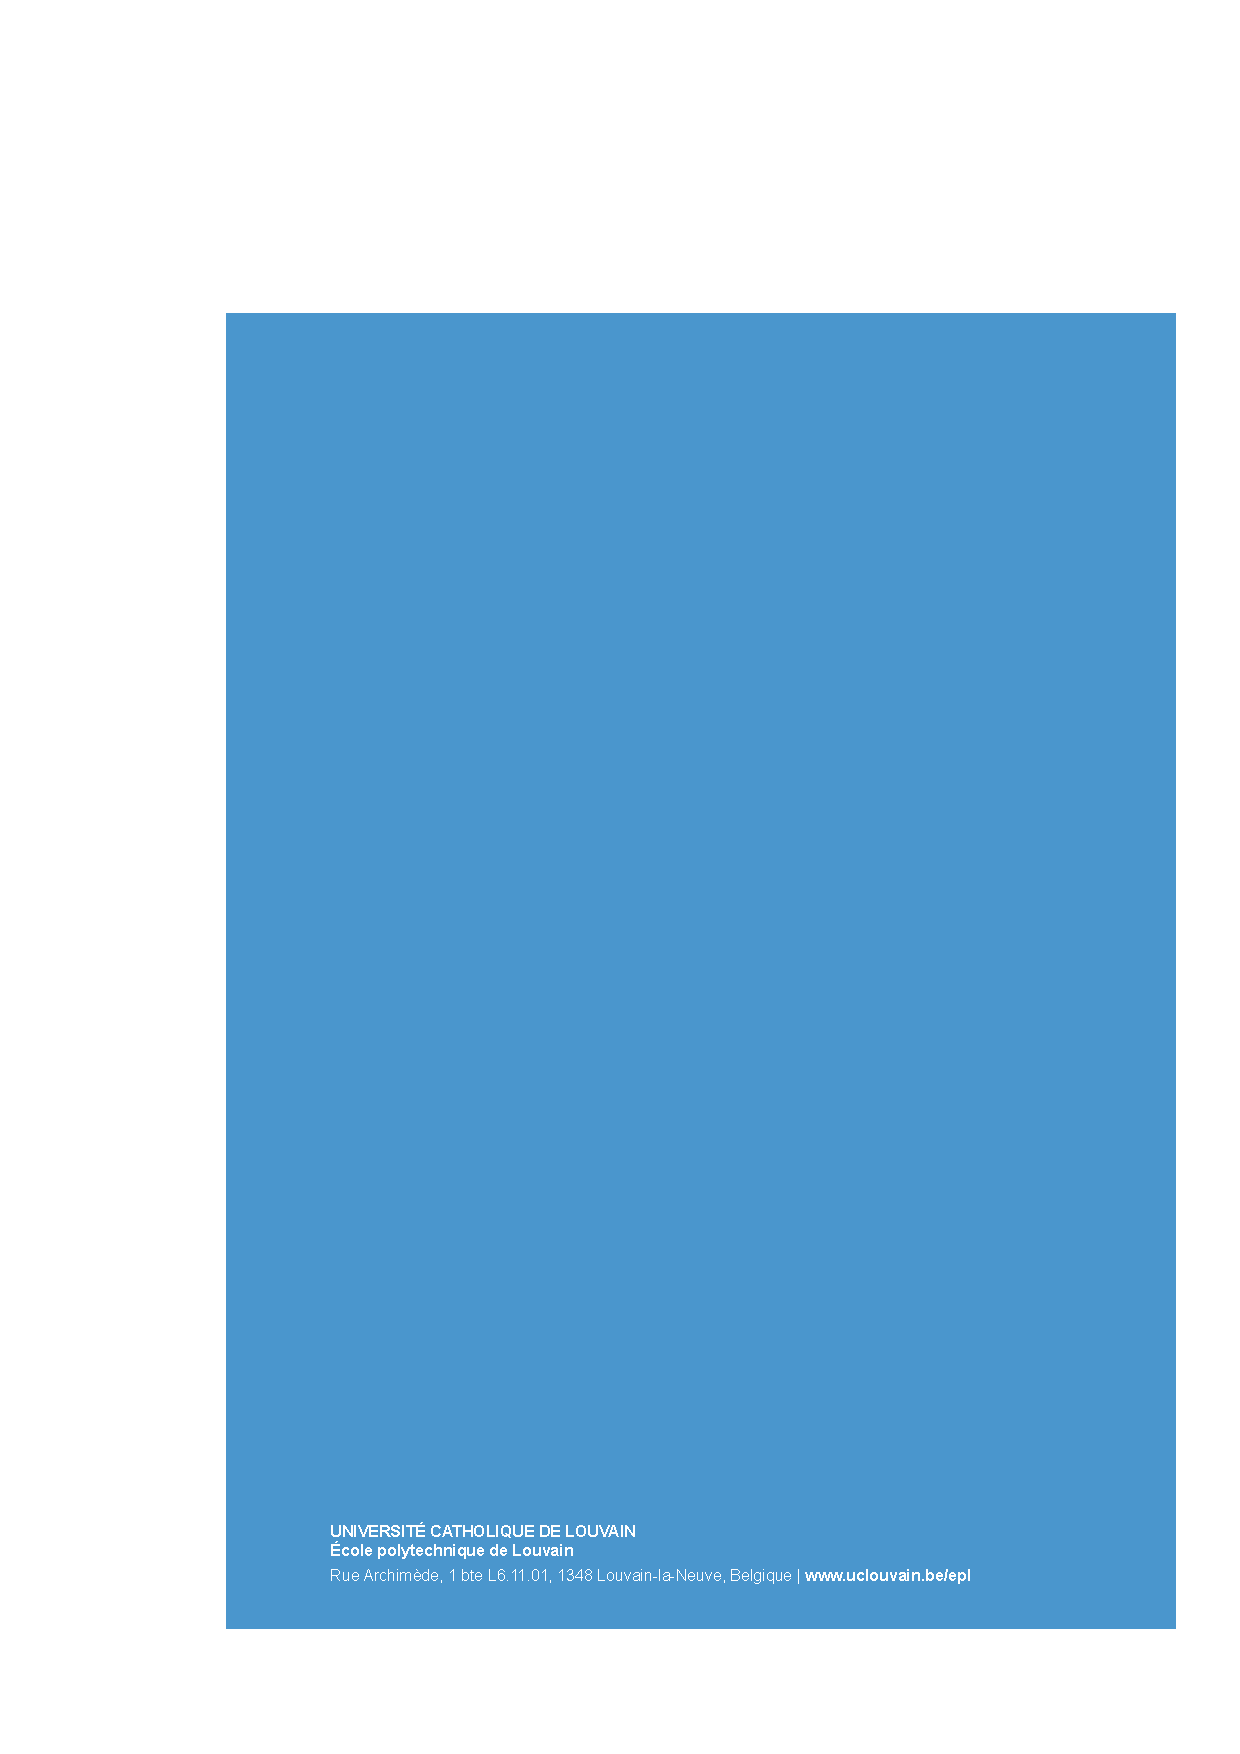
\includepdf[pages=-]{back_page.pdf}

\end{document}


    \draw[gray, thick] (2,0) -- (6,0);
    \draw[gray, thick, dotted] (-2, 0) -- (2, 0);
    \filldraw[black] (0,-1) circle (1pt);
    \draw[black] (0,-1) circle ({sqrt(5)});
    \draw[<->] (0, -0.1) -- (0, -0.9) node[midway, right] {$\Bar{z} + z^*$};
    \draw[<->] ({-sqrt(5)+0.1}, -1) -- (-0.1, -1) node[midway, below] {$R$};


    \begin{split}
        I_2(\mathbf{A}) &\coloneqq \frac{1}{2} \left[\Tr(\mathbf{A}^2) - \big(\Tr(\mathbf{A})\big)^2\right]
    \end{split}
    \quad \implies
    \begin{split}
        \dot \gamma &\coloneqq \sqrt{I_2(\gam)} = \sqrt{\frac{1}{2} \, \gam : \gam} = \sqrt{2 \mathbf{D} : \mathbf{D}}\\
        \tau &\coloneqq \sqrt{I_2(\boldsymbol\tau)} = \sqrt{\frac{1}{2} \, \boldsymbol\tau : \boldsymbol\tau}
    \end{split}
